\paragraph{Is there a trade-off between accuracy and robustness?}

    Although the existence of a trade-off between accuracy and robustness is commonly admitted, some works argue that ``Robustness is not inherently at odds with accuracy''\cite{yang2020closer}. We propose a unified consideration by stating that for a given train accuracy, robustness can be maximized up to a certain point, but allowing a lower train accuracy helps achieving a higher robustness. Finally one must keep in mind that this trade-off lives in the shade of generalization (see Section~\ref{sec:generalize}).

    \begin{figure}%[h]
        \centering
        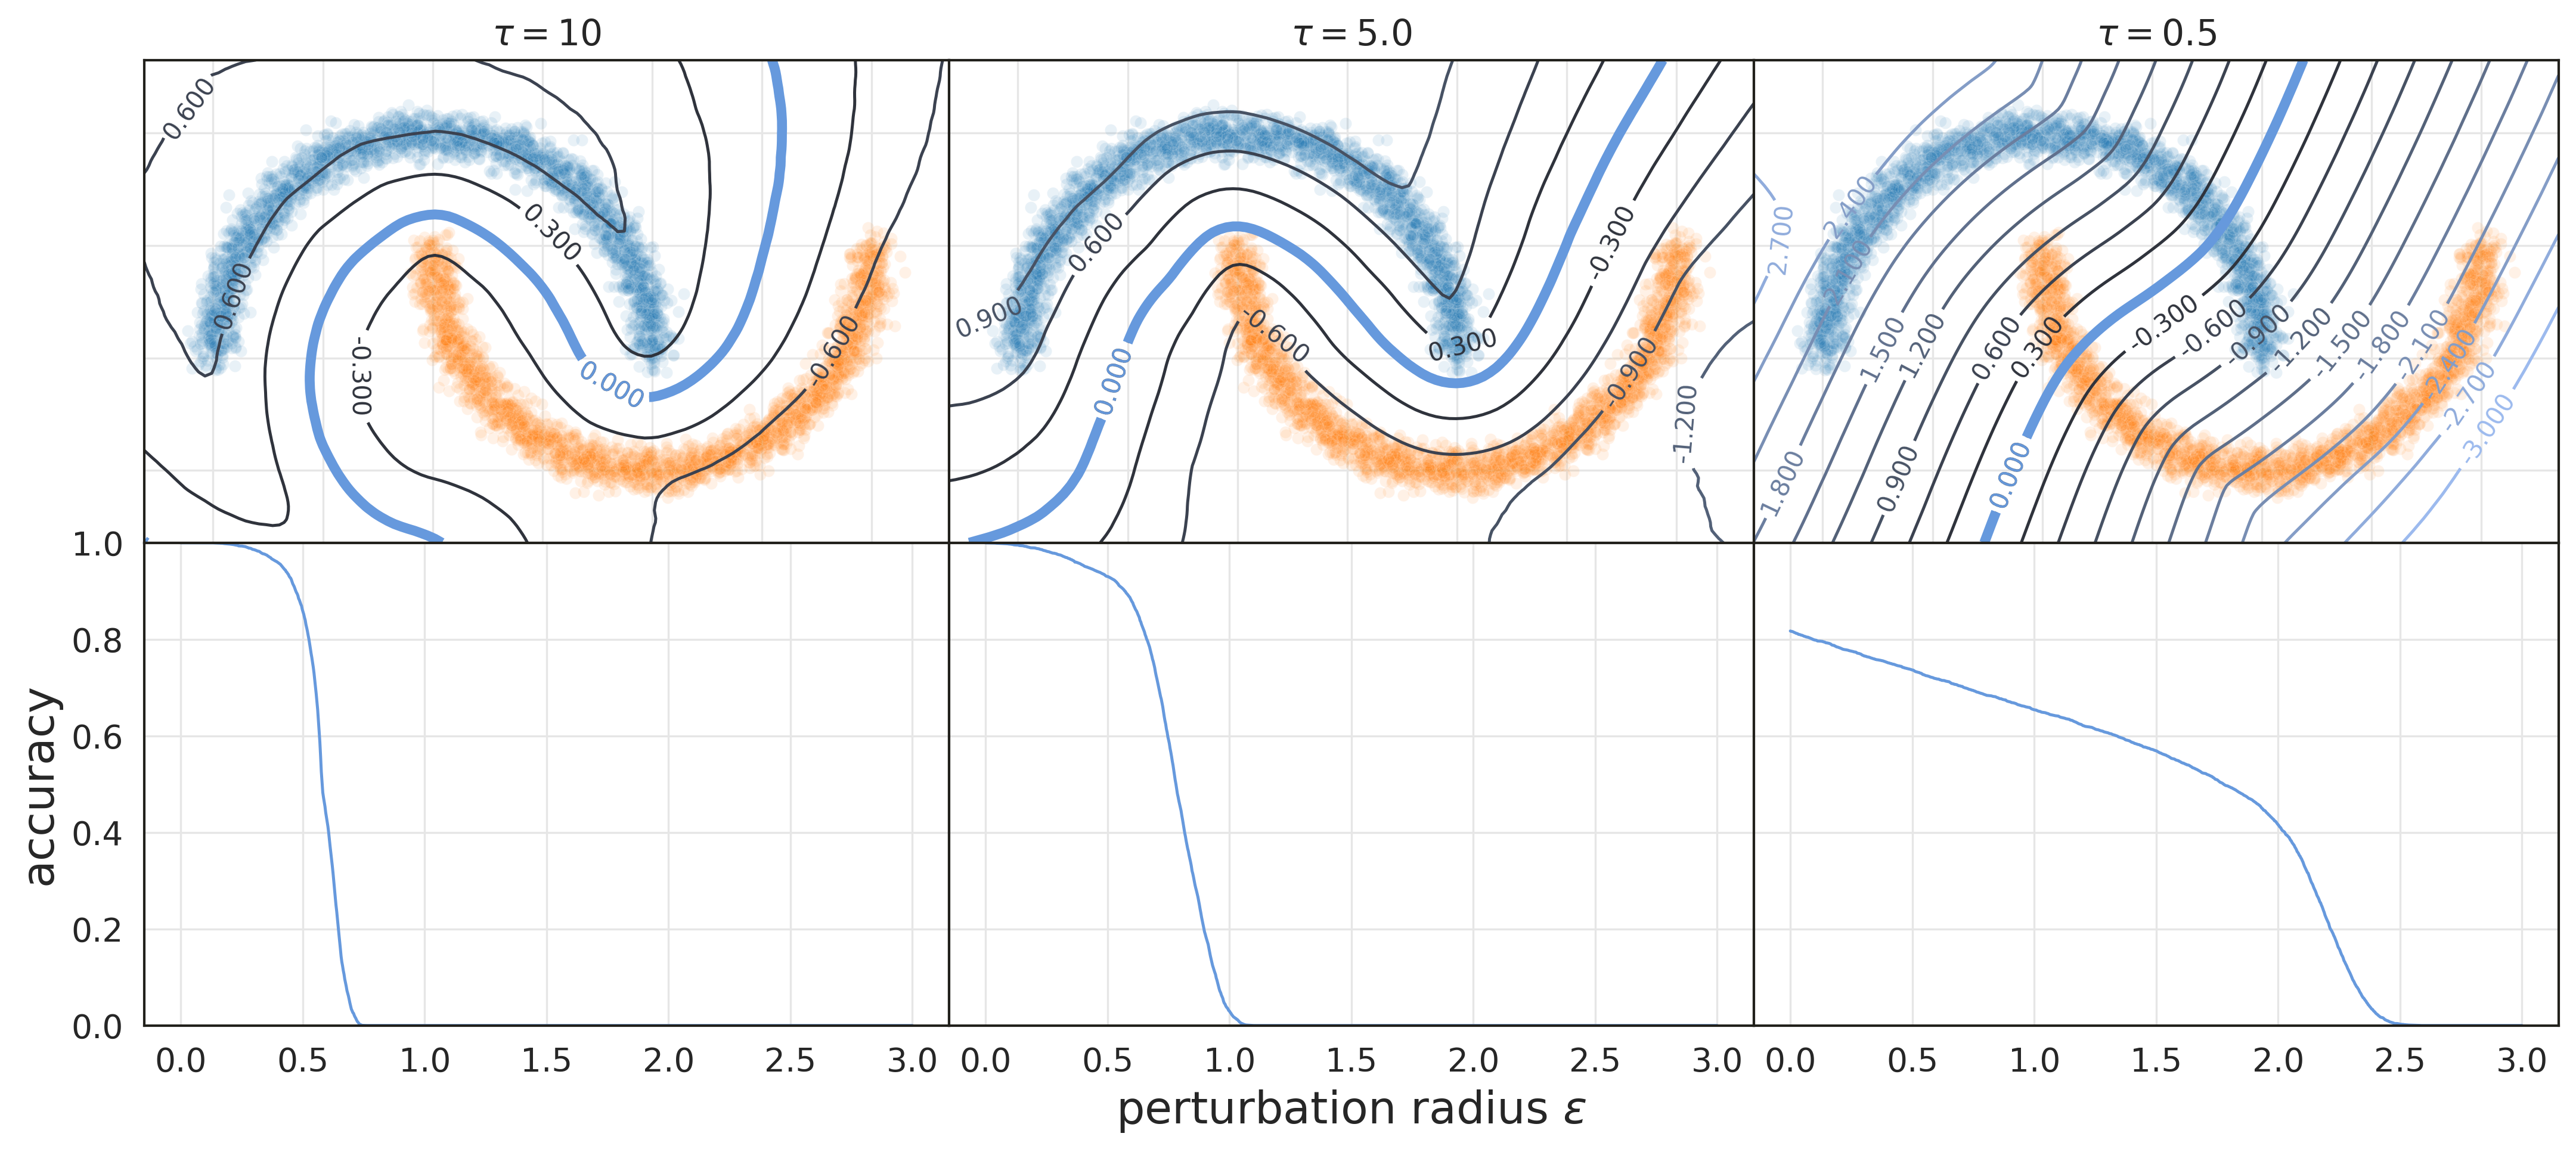
\includegraphics[width=0.8\textwidth]{images/acc_vs_rob/acc_vs_rob_2moons_cce.png}
        \caption{\textbf{Accuracy-robustness tradeoff:} Each network is optimal with respect to a certain criterion. The leftmost network is the most accurate at robustness radius $\epsilon\leq 0.3$, the rightmost maximizes the MCR at the cost of low clean accuracy. The center network corresponds to a compromise.% Influence of HKR parameters $\lambda,m$ on decision frontier $\partial$ (highlighted in red) on Two Moons dataset. Certifiable accuracy as function of perturbation radius in bottom row. %Weak and robust classifier on the left. Accurate and non robust classifier on the right. Accuracy-Robustness tradeoff in center.
        }
        \label{fig:twomoonstradeoff}
    \end{figure}

\subsection{Improving the robustness of the maximally accurate classifier}%Maximally robust accurate classifier}%\label{sec:robustness}  
    \label{max_acc}
      
    The Signed Distance Function~\cite{rousson2002shape} (SDF) (see Definition~\ref{def:nlctwoclasses} in Appendix~\ref{app:classificationpower}) associated to the frontier $\partial$ of Bayes classifier $b$ is the 1-Lipschitz function that provides the largest certificates among the classifiers of maximum accuracy. Moreover, those certificates are exactly equal to the distance of adversarial samples. Iterative gradient based attacks (see~\cite{chakraborty2018adversarial} and references therein) can succeed in one step: far from being a weakness, this may improve the interpretability of the model~\cite{dong2017towards,tomsett2018failure,ross2018improving}. 
    
    % is such that the certificates are exactly equal to the distance to these adversarial examples, and every gradient based attack (PGD, )
    % any empirical attack provides the same (optimal) adversarial examples, but also the network provides certificates exactly equal to the distance to these adversarial examples. 
      
    \begin{restatable}{corollary}{thightboundcertificate}\label{thm:thightboundcertificate}
        For the SDF($b$), the bound of Property~\ref{thm:certificates} is tight: $\epsilon=|f(x)|$. In particular $\delta=-f(x)\nabla_xf(x)$ is guaranteed to be an adversarial attack. The risk is the smallest possible. There is no classifier with the same risk and better certificates. Said otherwise the SDF($b$) is the solution to:
        \begin{equation}
            \begin{aligned}
                \max_{f\in\Lip}\min_{x\in\Xsub}&\min_{\substack{\delta\in\Reals^n\\ \sign{(f(x+\delta))}\neq \sign{(f(x))}}} \|\delta\|,\\
                \textrm{under the constraint } &  f\in\argmin_{g\in\Lip}E(\sign\circ g).\\
            \end{aligned}
        \end{equation}
        % where $\Risk(c)=E(c)-E(b)$ is the risk of the classifier, and where $b$ denotes the optimal Bayes classifier. 
    \end{restatable} % Dire que c'est LOWER bound
    
    The SDF($b$) cannot be explicitly constructed since it relies on the (unknown) optimal Bayes classifier. % We deduce that to train a \LipCl network that yields the best robustness certificates, we must aim to maximize $|f(x)|$.  
    
\subsection{Improving the accuracy of the maximally robust classifier}
    \label{max_rob}
    
    On the opposite side, we exhibit a family of classifiers with lower accuracy but with higher certifiable robustness. We insist that the quantity of interest is the \textit{certifiable robustness} $|f(x)|$ and not the \textit{true empirical robustness} $\epsilon$ (which can be higher). The former is computed exactly and freely, while the latter is a difficult problem for which only upper bounds returned by attacks are available. In the literature, the robustness is only evaluated on well classified examples. The certificate can be both interpreted as a form of ``confidence'' of the network, and as the minimal perturbations required to switch the class. Hence, we shall weight negatively this certificate for the examples that are misclassified since confidence in presence of errors is worse. For this reason, we propose in Definition~\ref{def:meancertifiable} a new metric called the Mean Certifiable Robustness (MCR).
      
    \begin{definition}[\textbf{Mean Certifiable Robustness -- MCR}]\label{def:meancertifiable}
        For any function $f:\Xsub\rightarrow\Reals\in\LipCl$ we define its weighted mean certifiable robustness $\mathcal{R}_{(P,y)}(f)$ on class $P$ with label $y$ as:  
        \begin{equation}
            \begin{aligned}
                \mathcal{R}_{(P,y)}(f)&\defeq\Expect_{x\sim P}[{\mathds{1}\{yf(x)>0\}|f(x)|}]+\Expect_{x\sim P}[{-\mathds{1}\{yf(x)<0\}|f(x)|}]=\Expect_{x\sim P}{yf(x)}.
            \end{aligned}
        \end{equation} 
    \end{definition}  % expliquer pk ça sert à rien pour les AllNet (pas de certificat)
      
    We can readily see from the definition that the classifier with highest MCR for class $P$ is the constant classifier $f=y\times\infty$. The interest of this notion arises when we consider minimizing the loss function $\Loss^{W}(f(x),y)\defeq-yf(x)$, i.e when looking for classifier with the highest MCR.   
      
    \begin{restatable}{property}{mcriswass}{\normalfont\textbf{Wasserstein classifiers (i.e WGAN discriminators) are optimally robust}.}\label{thm:mcriswass}
        The minimum of $\Loss^{W}(f(x),y)$ over $P$ and $Q$ is the Wasserstein-1 distance~\cite{villani2008optimal} between $P$ and $Q$ according to the Kantorovich-Rubinstein duality:
        \begin{equation}\label{eq:wassdef}
            \max_{f\in\text{Lip}_1(\Xsub,\Reals)}\mathcal{R}_{(P,+1)}(f)+\mathcal{R}_{(Q,-1)}(f)=\min_{f\in\Lip}\Expect_{\Prob_{XY}}[\Loss^{W}(f(x),y)]=\Wasserstein_1(P,Q).
        \end{equation}
    \end{restatable}  % parler des WGAN discriminators
    
    Even though the minimizer of $\Loss_{W}(f(x),y)$ can have low accuracy, it has the highest MCR. Interestingly, the minimizer $f^{*}$ of equation~\ref{eq:wassdef} is invariant by translation: $f^{*}-T$ is also a minimizer for any $T\in\Reals$. When $T\rightarrow\infty$ (resp. $-\infty$) the classifier has $100\%$ recall on $Q$ (resp. $P$), and $0\%$ on $P$ (resp. $Q$). Does it always exist $T^{*}$ with $100\%$ accuracy overall? Sadly, even when the $P$ and $Q$ have disjoint support, the answer is no. We precise this empirical observation of~\cite{serrurier2020achieving} in Proposition~\ref{thm:weakwass}.
      
    \begin{restatable}{proposition}{weakwass}{\normalfont\textbf{WGAN discriminators are weak classifiers}.}\label{thm:weakwass}
        For every $\frac{1}{2}\geq\epsilon>0$ there exist distributions $P$ and $Q$ with disjoint supports in $\Reals$ such that for any optimum $f$ of equation~\ref{eq:wassdef}, the error of classifier $\sign\circ f$ is superior to $\frac{1}{2}-\epsilon$.
    \end{restatable}  
    Note that this minimum also invariant by dilatation: any \textit{finite} upper bound $L$ can be chosen for Equation~\ref{eq:wassdef} (see Appendix~\ref{sec:krunit}).
      
    % In the next section we answer the remaining question: which loss should we choose to maximize accuracy \textit{and} certifiable robustness ?
    % In the next section we answer the remaining question: which loss should we chose to achieve this goal ?  
% \begin{figure}
    %     \centering
    %     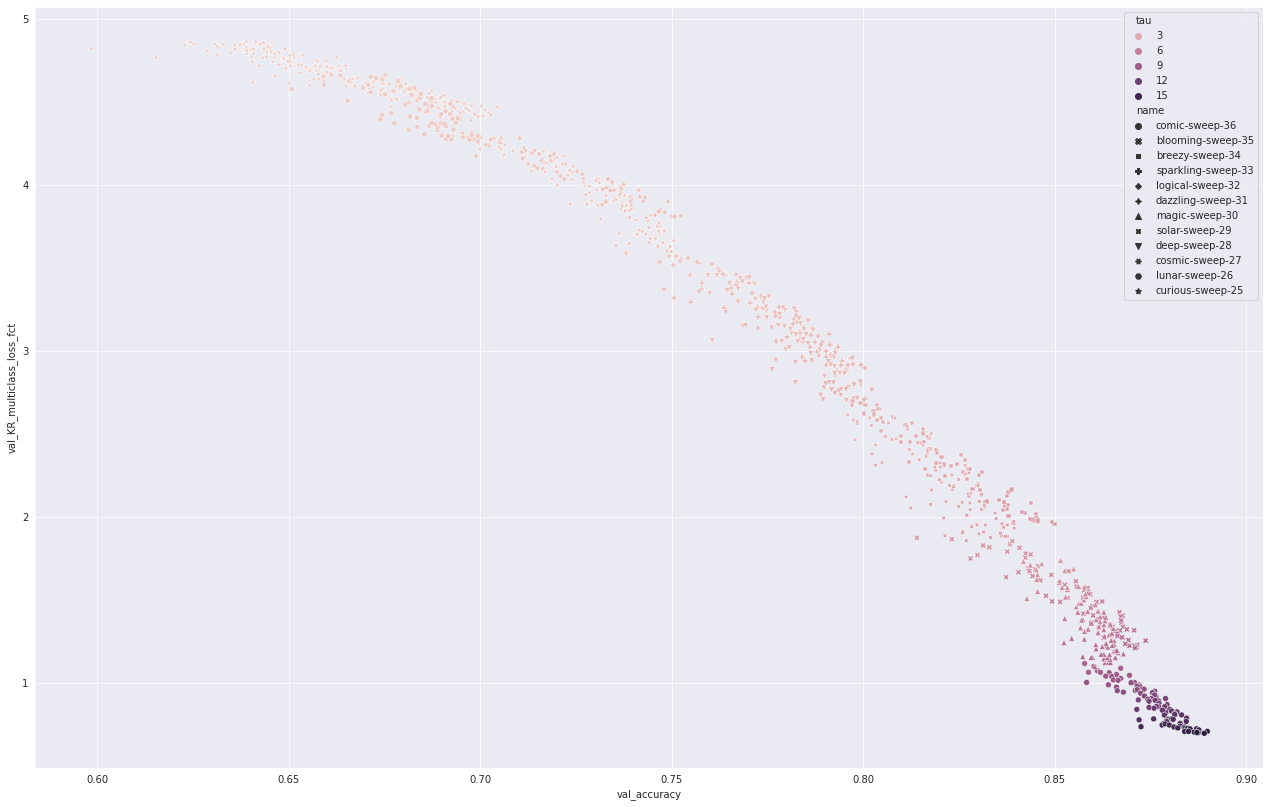
\includegraphics[width=0.8\textwidth]{images/pareto/pareto_placeholder.png}
    %     \caption{\textbf{The cross-entropy's temperature controls the trade-off between accuracy and robustness.} The same \LipCl architecture is trained numerous times with cross-entropy on CIFAR10. For different $\tau$ values (points), the clean accuracy (x-axis) and the robust accuracy (\thib{choose metric} on y-axis) are reported. Increasing $\tau$ increases the network accuracy, but also decrease its robustness.}
    %     \label{fig:ce_pareto}
    % \end{figure}

    % \begin{figure}%[h]
    %     \centering
    %     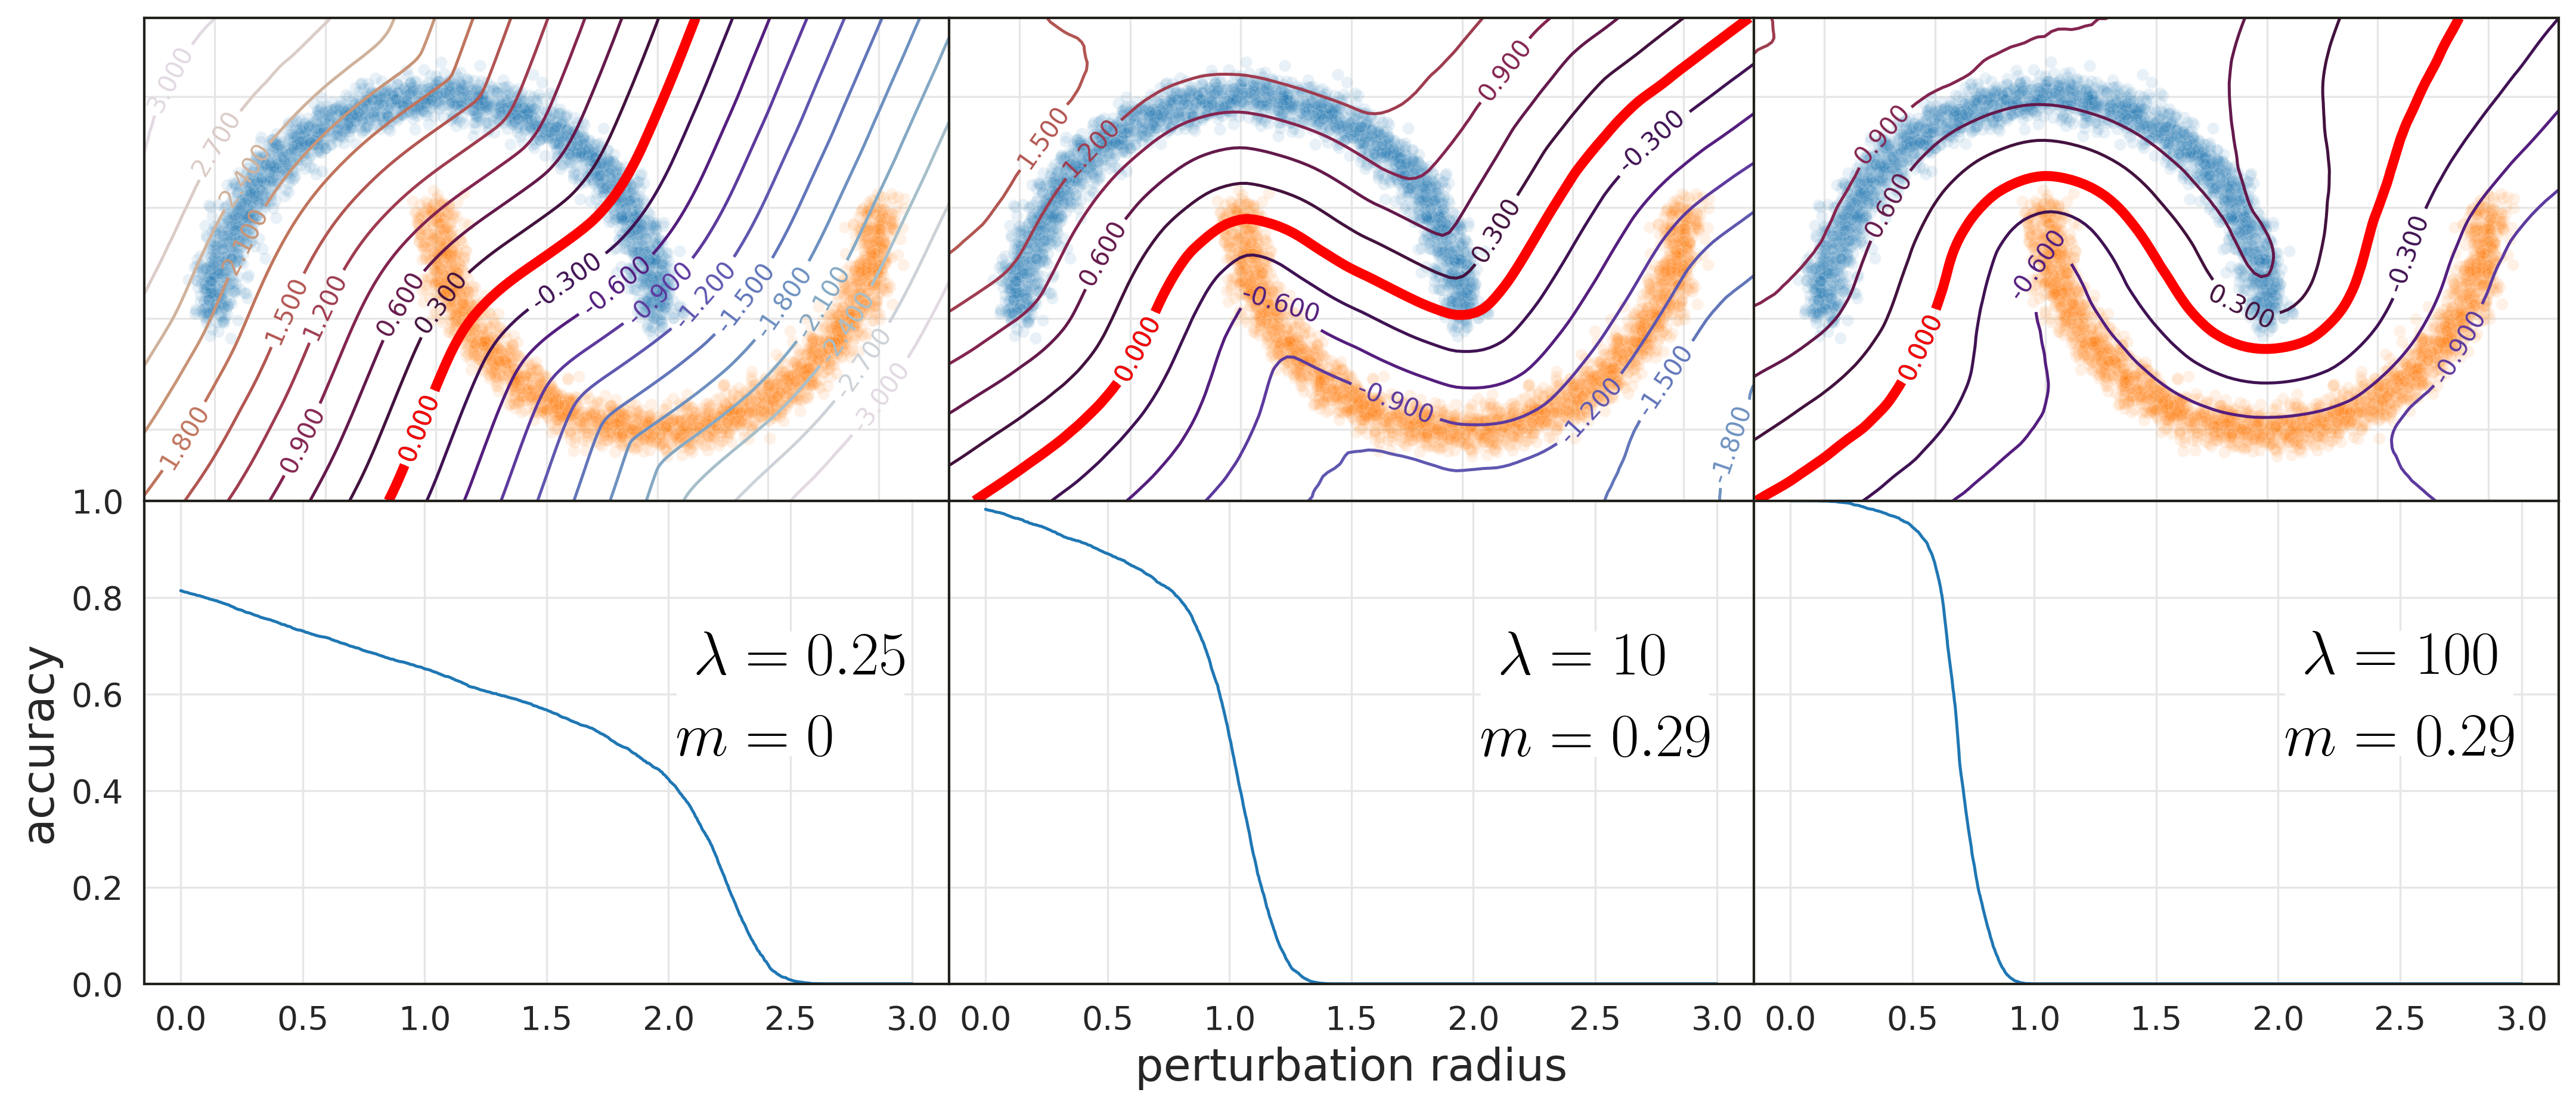
\includegraphics[width=0.85\textwidth]{images/acc_vs_rob/acc_vs_rob_2moons_bis.png}
    %     \caption{Influence of HKR parameters $\lambda,m$ on decision frontier $\partial$ (highlighted in red) on Two Moons dataset. Certifiable accuracy as function of perturbation radius in bottom row. %Weak and robust classifier on the left. Accurate and non robust classifier on the right. Accuracy-Robustness tradeoff in center.
    %     }
    %     \label{fig:twomoonstradeoff}
    % \end{figure}
    \subsection{Controlling the accuracy/robustness tradeoff with loss parameters}
    
    Now that the extrema of the accuracy robustness tradeoff were characterized in \ref{max_acc} and \ref{max_rob}, is yet to be answered if it is possible to control this tradeoff using conventional loss (and its parameters, as introduced in \ref{sec:lipclminexists}).
    
    Interestingly, observe that $\Loss^{bce}_{\tau}(f(x),y)=\log{2}-\frac{y\tau f(x)}{2}+\mathcal{O}(\tau^2 f^2(x))$ so when $\tau\rightarrow 0$ we get:
        $$\min_{f\in\text{Lip}_1(\Xsub,\Reals)}\frac{4}{\tau}\left(\Expect_{(x,y)\sim P_{XY}}[\Loss^{bce}_{\tau}(f(x),y)]-\log{2}\right)=-\Wasserstein_1(P,Q).$$
    In the limit of small temperatures, the BCE minimizer essentially behaves like the classifier of the highest MCR (see Figure~\ref{fig:pareto_hkr} and Appendix~\ref{ap:bceot}). Similarly, the HKR loss $\Loss^{hkr}$ introduced in~\cite{serrurier2020achieving} for \LipCl training allows fine grained control of the accuracy-robustness tradeoff: % (see Appendix~\ref{ap:pareto}): 
    \begin{equation}~\label{eq:hkrdef}
        \Loss^{hkr}_{m,\alpha}(f(x),y)=\Loss^W(f(x),y)+\alpha\Loss^H_{m}(f(x),y)=-yf(x)+\alpha\max{(0, m - yf(x))}.
    \end{equation}
    % In the limit of high temperatures, BCE behave like the 0-1 loss, i.e the empirical accuracy. We saw that BCE requires tuning of $L$ or $\tau$. Hinge allows high accuracy but does not optimize the certificates.
    
    % \begin{definition}[Hinge Kantorovich-Rubinstein (HKR)]\label{def:hkr}
    % The combination of Hinge with KR dual potential is the \textbf{Hinge Kantorovich-Rubinstein (HKR)} loss:
    % \begin{equation}~\label{eq:hkrdef}
    %     \Loss^{hkr}_{m,\lambda}(f(x),y)=\Loss^W(f(x),y)+\lambda\Loss^H_{m}(f(x),y)=-yf(x)+\lambda\max{(0, m - yf(x))}
    % \end{equation}
    % \end{definition}
    % Its minimization is a regularized optimal transport (OT) problem~\cite{serrurier2020achieving}.
    We recover $\Wasserstein_1$ behavior for $\alpha=0$, and hinge $\Loss^H_{m}$ behavior for $\alpha\rightarrow\infty$, in a fashion that reminds the role of $\tau$ for $\Loss^{bce}$.
    
    A key takeaway is that BCE, HKR and hinge loss have parameters that allow to control the accuracy robustness tradeoff, reaching on one side the maximum robustness of MCR, and the accuracy of unconstrained networks on the other. Empirically this tradeoff is observed as a Pareto front with accuracy on one axis, and robustness on the other. Figure \ref{fig:pareto_hkr} shows this on the CIFAR10 dataset using the $\epsilon$ robustness as robustness measures (other robustness measure yield similar observations, see fig \ref{fig:pareto-avg} and \ref{fig:pareto-MCR}).
    
    In conclusion, these last two sections demonstrate that restraining networks to be in \LipCl does not impact the classification capabilities while providing certificates of robustness; however, for these networks the loss parameters play an important role in this trade-off. % (Figure~\ref{fig:pareto_hkr}).%however loss parameters must be chosen carefully.   

    \begin{figure}
        \centering
        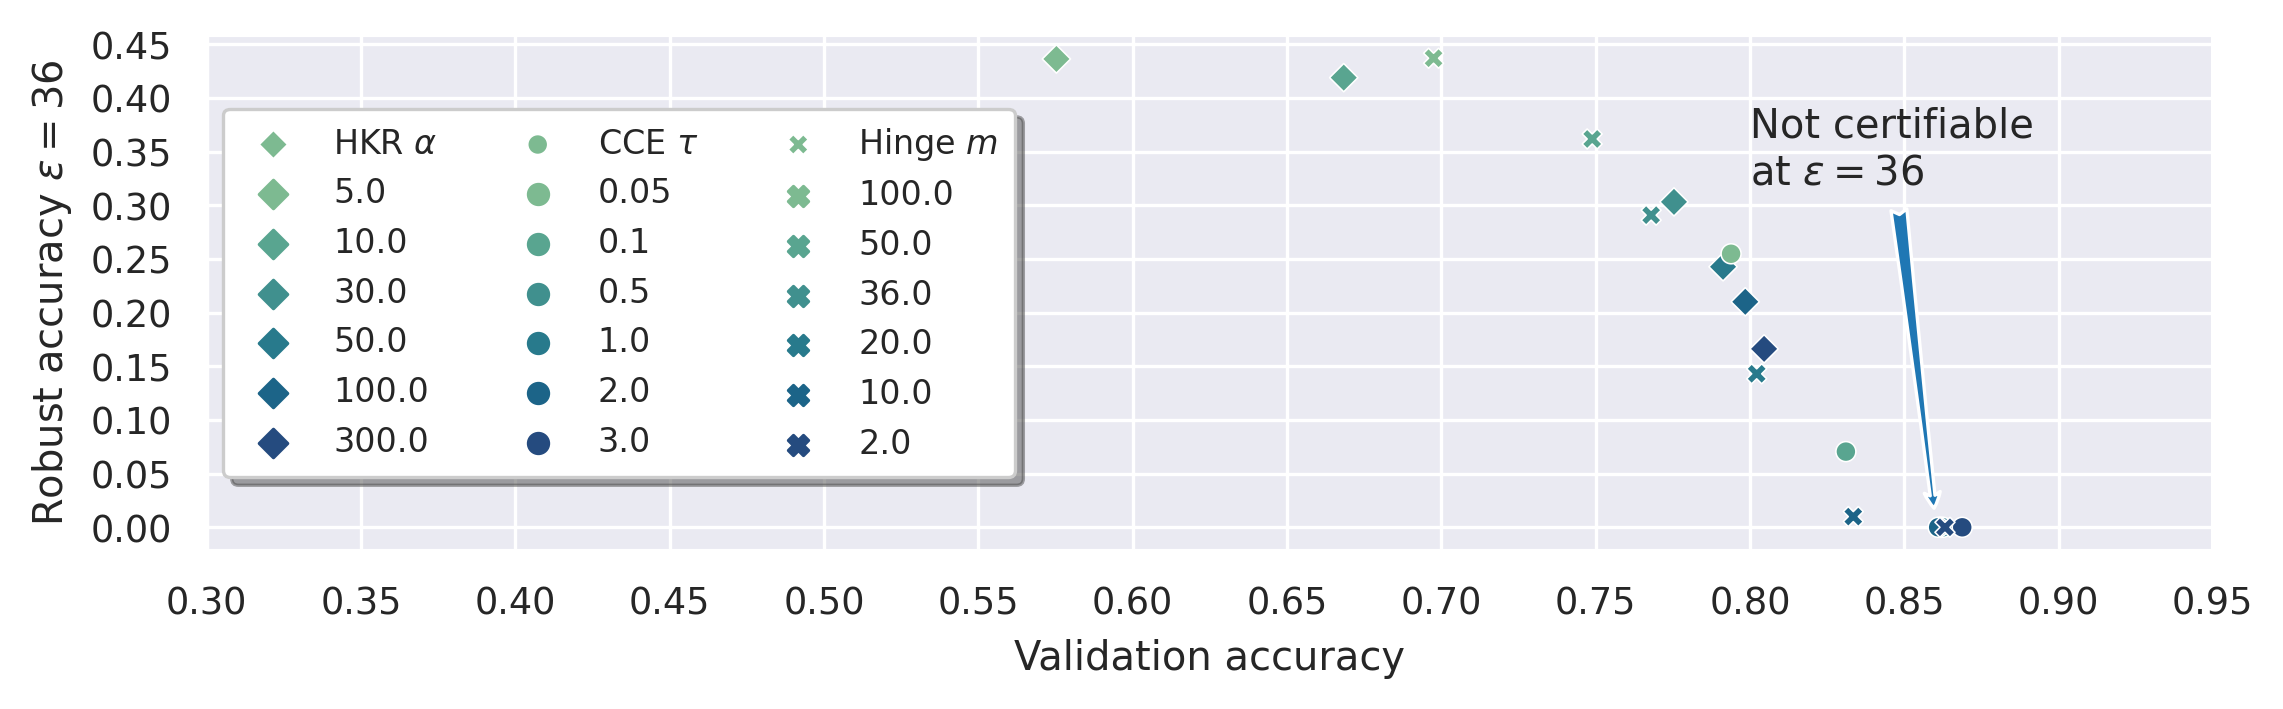
\includegraphics[width=0.95\textwidth]{images/pareto/T2.png}
        \caption{\textbf{Accuracy-Robustness trade-off on CIFAR10 with Hinge, HKR and Categorical Cross-Entropy (CCE) hyper-parameters.} Overall, for a given network architecture, a Pareto front appears between clean accuracy and robust accuracy. We move along it by tuning the parameters of each loss. We trained small \LipCl \textit{CNNs} (0.4M params) with basic data augmentation (see appendix~\ref{ap:pareto} for detailed experimental setting).}%\thib{HKR with m=20 in appendix}
        \label{fig:pareto_hkr}
    \end{figure}
